\chapter{\textit{Waisda?}:Open-source Video Labelling Game}\label{chap:waisda}

\begin{quotation}
\noindent 
In this chapter we shall describe in more detail the video labelling game \textit{Waisda?} and how it can be exploited as a crowsourcing tool for collecting user-generated tags for video clips. We shall also outline the results and efforts from this thesis that had an impact on the development of \textit{Waisda?}.

This chapter is based on the paper entitled \textit{Waisda?: video labeling game} which was presented at Proceedings of the 21st ACM international conference on Multimedia, held in Barcelona, Spain. The paper is authored by Michiel Hildebrand, Maarten Brinkerink, Riste Gligorov, Martijn Van Steenbergen, Johan Huijkman, and Johan Oomen.
\end{quotation}

\section{Introduction}

In essence, \textit{Waisda?} is a Game With A Purpose (GWAP). GWAPs are a human-based computation technique in which a computational process performs its function by outsourcing certain steps to humans in an entertaining way \cite{Ahn:2006:GP:1155311.1155342,gwap}. The crux of this approach is the realization that humans are better than computers in certain tasks. For example the computers still lack the basic conceptual intelligence or perceptual capabilities required for carrying out the task of labelling random images and videos \cite{Ahn:2006:GP:1155311.1155342}. In fact, the first example of a GWAP, the ESP Game created by Luis von Ahn, labels images on the Web by harnessing the capabilities of the players. The ESP game randomly pairs up two players with the task to describe images. Players don't know who their partner is, nor can
they communicate with each other. The only thing partners have in common is an image they can both see.
When both players provide the same label for an image, they score points and proceed to the next image. The labels entered by both users are associated to the image as metadata. In other words, the consensus among players is a mechanism to ensure the quality and consistency of the labels. The same design principles are applied in \textit{Waisda?} as well. \textit{Waisda?} is a multi-player labelling game where players compete with each other by tagging streaming video. The players score points by entering the same tag as one of the other players within a ten seconds interval. As a result, the video that is tagged in the game is annotated with the matched tags which are anchored to the time points in the video when they were entered.

\textit{Waisda?} was conceived by the Netherlands Institute for Sound and Vision (S\&V) and the VU University Amsterdam in the context of the Dutch project Images for the Future\footnote{\url{http://imagesforthefuture.com/}} and the European research project PrestoPRIME, as an open-source crowdsourcing tool that can be deployed by multimedia collection owners as crowdsourcing initiatives to annotate their collection items. The development of the software was contracted to Q42, a Dutch internet development company\footnote{\url{http://q42.com/}}. The Netherlands Institute for Sound and Vision in cooperation with Dutch broadcasters deployed \textit{Waisda?} in two consecutive pilots featuring historical archive material as well as recent TV episodes from Dutch shows. The first pilot of the game run from May 2009 until January 2010 and produced over $420,000$ user tags. The follow up analyses of the collected tags \cite{Annelies,ecir} and user evaluations suggested potential areas of improvement. Considering the acquired experience and insights, S \& V launched a second pilot of the game\footnote{At the time of writing, the game is deployed online and can be accessed at \url{http://woordentikkertje.manbijthond.nl/}.} which featured several improvements, albeit the basic idea of the temporal tag agreement is preserved. The two pilots together resulted in more than a million tags describing thousands of videos. In fact, the studies described in Chapter \ref{chap:kcap} and \ref{chap:ecir} are based on the data collected in the first and the second pilot, respectively.

The open source version of Waisda? enables maintainers of an online video collection to start their own crowdsourcing initiative for time-based annotations. In particular, we believe that Waisda? is a valuable tool for cultural heritage institutions, as it provides a novel and engaging way for the public to access and interact with the audiovisual material.

In the rest of this chapter we shall describe the gameplay and the user interface of \textit{Waisda?}, explain the software architecture, and give examples of successful deployment of \textit{Waisda?} by third parties. In the final section we outline the results and efforts from this thesis that had an impact on the development of \textit{Waisda?}.

\section{Gameplay and User Interface}
The gameplay of Waisda? is straightforward: the player first selects a video from the \textit{Homepage}, plays the \textit{Game} by watching the video and entering tags, and finally studies the results in the \textit{Game recap} to learn what he/she can improve in future games.

\subsection{Homepage}
Figure \ref{homepage} shows the homepage of \textit{Waisda?}, with six videos that the user can choose from. A player starts a game by selecting one of these videos. To give other players the opportunity to join the game, the player first enters the waiting room. In the waiting room the players can study the game
instructions and after 20 seconds the game is automatically started. On the homepage the games that are waiting for players are shown at the bottom right. Players can quickly join a game by selecting one of the entries.
The homepage also contains the basic instructions that prepare the user for the game. To honour the top players, and motivate the other players, the homepage contains a leaderboard that displays the top players of the week. To engage the players with the purpose of the game a notification at the top of the page shows the total number of tags that were entered into the system, and the users contribution to this total. This part of the page also contains the links to register and login. Games can be played without registering, but only for registered players the score is maintained in the player’s profile. To explain the potential of the contributed tags, the page contains a tag cloud with the most popular tags. By selecting a tag the user can navigate the video collection. Finally, the bottom of the page has space reserved for logos and navigation links to additional pages, such as an about page or a page with the terms of use.

\begin{figure}[t!]
\centering
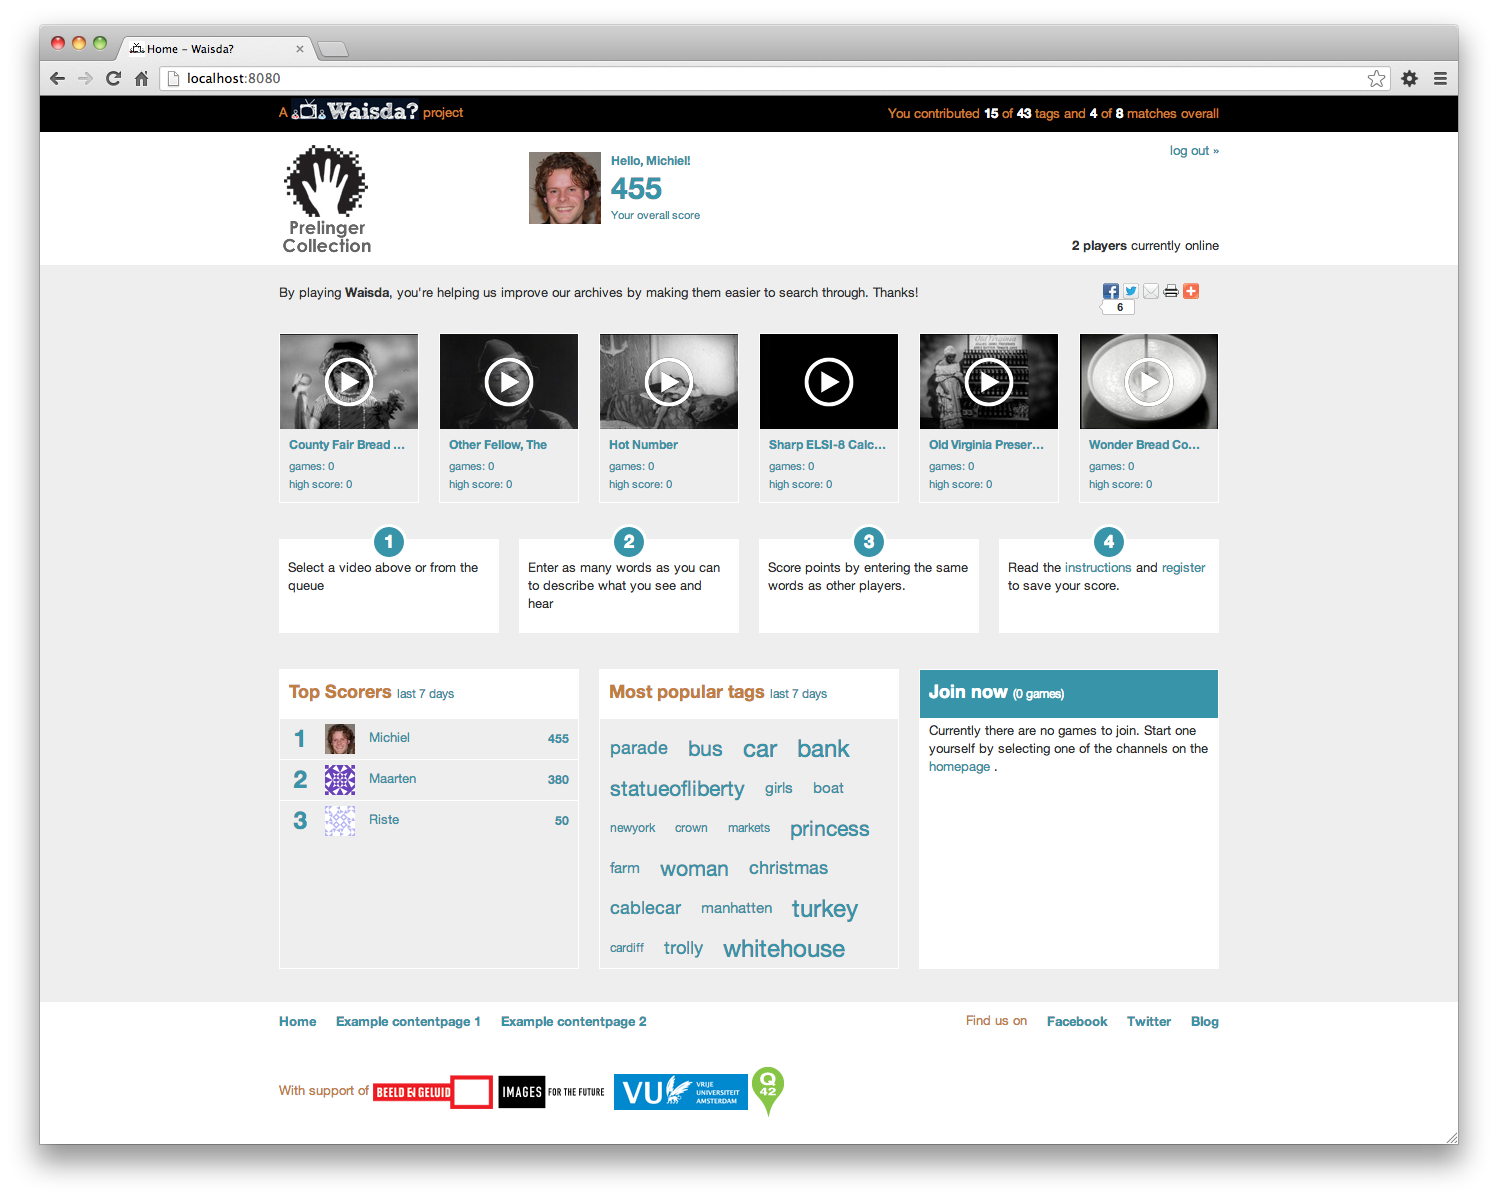
\includegraphics[width=\columnwidth]{figs/homepage} 
\caption{Screenshot of the Waisda? homepage with public domain video clips from the Prelinger Archives.}
\label{homepage}
\end{figure}

\subsection{Game}\label{sec:waisda-game}

Figure \ref{game} shows the game page of \textit{Waisda?}. It contains a video player and below it a text-entry field. When the player enters the game page the video automatically starts playing, the text-entry field receives focus, and the player can start entering tags. The right side of the page contains the score board. It consists of the current score of the player, the current rank and a listing with all tags entered by the player.
The tags are displayed with their score and an icon indicating the type of match and the tag type (person, location etc.).

\textit{Waisda?} uses a scoring mechanism to motivate users to (keep) playing the game, and reward them for entering specific types of tags. The basic scoring mechanism is tag agreement, two players entering the same tag. From the perspective of the video collection tag agreement provides a mechanism to improve the quality, tags that are entered by more than one user are less likely to contain spelling errors and are more likely to provide a trustworthy description of the video. Tags are considered a match if they are syntactically
the same after normalization and entered within a ten second interval of each other. The details of the normalization procedure are explained in the documentation. The matching procedure can be extended by importing tag similarity lists. For example, tags can be matched semantically by importing synonym lists, and specific tags (e.g. Labrador) can be matched with more generic tags (e.g. Dog) by importing word pairs derived from the hierarchical structures of linguistic or domain specific thesauri.

\textit{Waisda?} also contains a mechanism to reward players for entering specific types of tags. For example, when tagging videos in the art domain the names of artists are important. By importing a dictionary with artist names \textit{Waisda?} detects these tag types and rewards the players additional points.

As we can not expect that there are always sufficient users active at the same time, the scoring mechanism of \textit{Waisda?} also motivates users to play alone. In this case a player scores points by matching with the tags that were entered for the same video in previous games. To ensure players not
only tag in the most obvious ways, the scoring mechanism of \textit{Waisda?} also motivates players to \textit{pioneer} new tags. A player enters a pioneer tag when this tag is not entered for this video before, and afterwards it is matched with tags entered by other players (in the same or a later game).

\begin{figure}[t!]
\centering
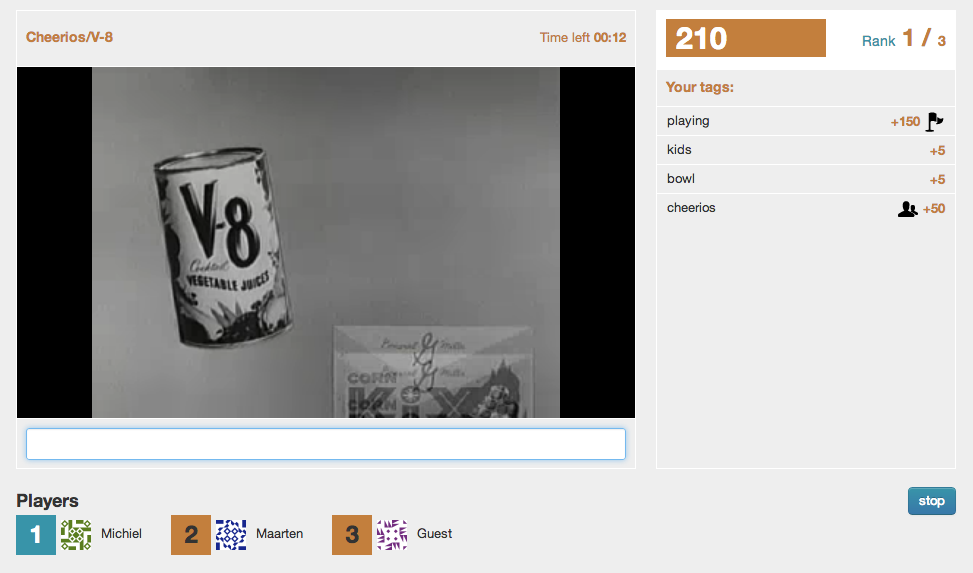
\includegraphics[width=\columnwidth]{figs/game} 
\caption{Screenshot of the Waisda? game page with public domain video clip from Preligner Archives.}
\label{game}
\end{figure}

\subsection{Game Recap}

When the video ends the user is automatically redirected to the game recap (see Figure \ref{recap}). On this page the user can investigate his/her performance, learn about the details of the scoring mechanism and the behaviour of other players. The game recap consists of two parts. The tag statistics, placed on the left part of the screen,give an overview of the number of tags entered by the player in different categories, including the number of matched tags, pioneer tags and specific types of tags. The tag details, placed on the right part of the screen, are listing of all the tags entered by the player. The listing is similar as the one provided in the game, but includes information about other player in the game, if any, who entered the same tag within a ten seconds interval i.e. a tag match has been achieved.

\begin{figure}[t!]
\centering
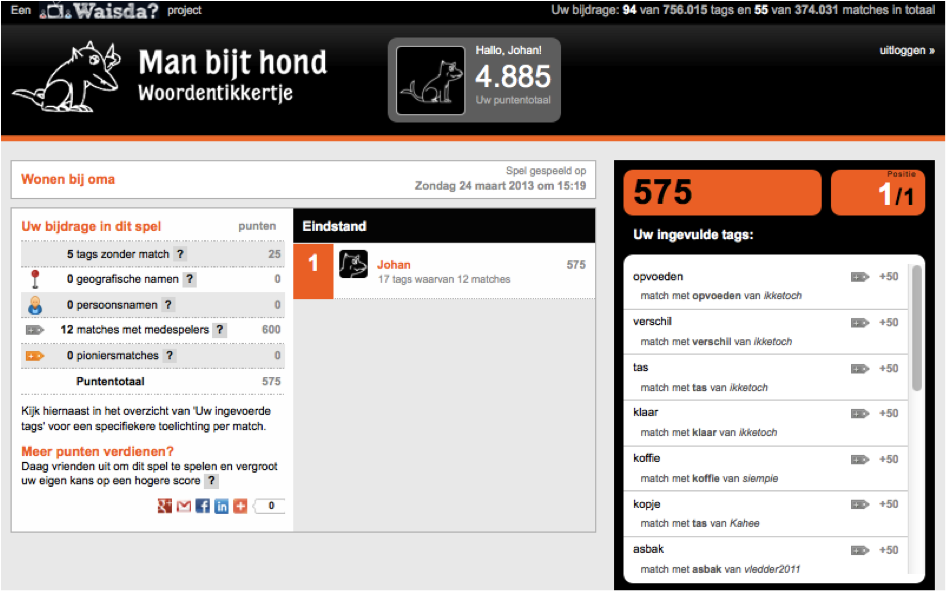
\includegraphics[width=\columnwidth]{figs/recap} 
\caption{Screenshot of the Waisda? \textit{game recap} after a successfully finished game.}
\label{recap}
\end{figure}

\section{Implementation}
\textit{Waisda?} is an open source crowdsourcing tool that has been designed and implemented as a 3-tier web application. The backend application logic is implemented in the Spring Framework\footnote{\url{http://spring.io/}}, which at the time of writing is one of the most widely used open source Java application frameworks. The application is backed by a MySQL\footnote{\url{http://www.mysql.com/}} database which is accessed via the Java Persistence API and Hibernate\footnote{\url{http://hibernate.org/}}. The user interface (UI) is rendered using the Java Server Page (JSP) technology. The UI consists of HTML, JavaScript, and CSS. jQuery and Twitter Bootstrap are used as the JavaScript and CSS libraries. The dynamic
stylesheet language LESS is used to allow easy configuration of the presentation style.

The Waisda? source code and documentation is available from Github \url{http://github.com/beeldengeluid/waisda}. The building, installing and running or the \textit{Waisda?} source code is handled by Maven\footnote{\url{http://maven.apache.org/}} which is a open-source software project management tool developed by the Apache Foundation. The getting started section of the documentation contains instructions to setup a deployment using videos from the Prelinger archive\footnote{\url{http://archive.org/details/prelinger}}.

\subsection{Backend}
After installation the maintainer has to populate the database with videos and optionally with dictionaries and similarity lists. A \textit{video} has a title, description, source URL, key frame URL, duration and video player type. There are currently two types of video players supported: the JWPlayer (HTML5 and Flash), and the NPO player (Silverlight). The latter is used to play content from Dutch public broadcasting associations. Each video in the project specifies which of the two players it would like to use, in combination with the parameters required for the players. To facilitate more robust scoring schemes auxiliary resources like dictionaries and similarity lists can also be used. As long as the data format is valid, the party that deploys the game is free to use any resources it pleases. A \textit{dictionary} is a set of word-type pairs which is used to reward additional points for specific types of tags. Examples are names of celebrities and names of geographical locations. A \textit{similarity list} is a set of word-word pairs which is used to extent the default syntactic tag matching with semantic similarity matching. Examples are synonym pairs or words that are hierarchically related (specific-generic).

\begin{figure}[t]
\centering
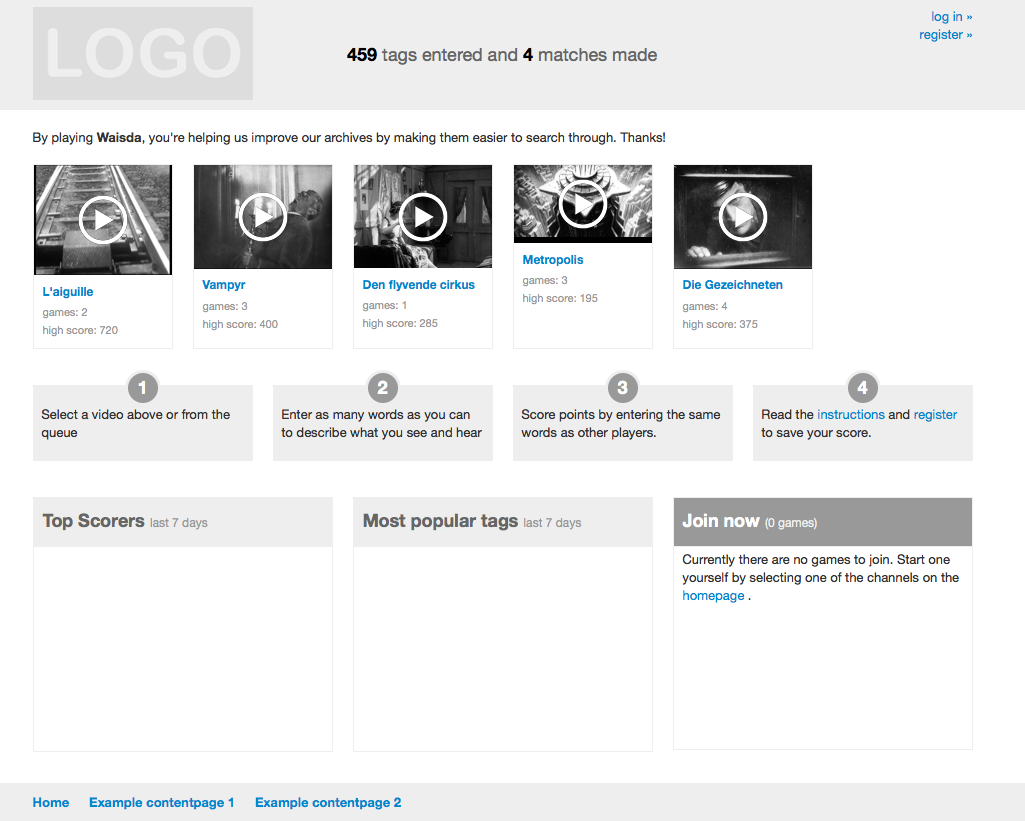
\includegraphics[width=\columnwidth]{figs/waisdastripped} 
\caption{Screenshot of the default user interface of Waisda? stripped of all branding and styling.}
\label{waisdastripped}
\end{figure}

\begin{figure}[t]
\centering
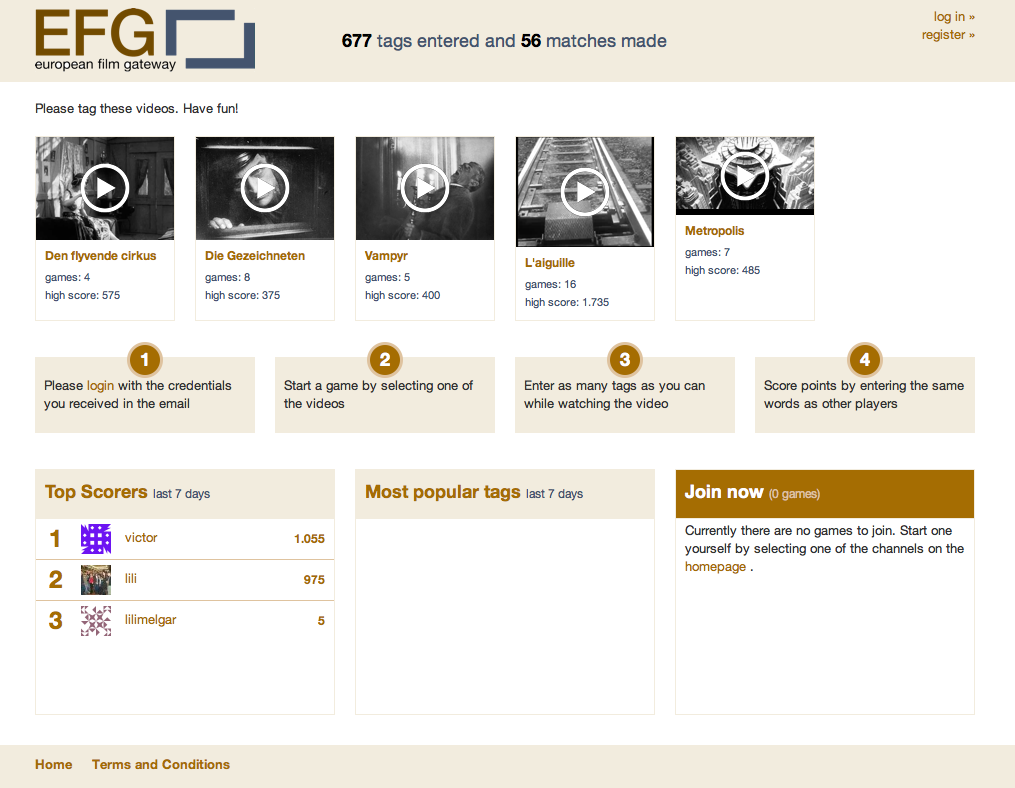
\includegraphics[width=\columnwidth]{figs/waisdaefgtheme} 
\caption{Screenshot of an experimental setup of Waisda? for the European Film Gateway (EFG). It is configured with five videos and the user interface contains a logo and an EFG colour scheme.}
\label{waisdaefgtheme}
\end{figure}

\subsection{Frontend}
The default user interface of \textit{Waisda?} is completely functional. In addition, basic branding and styling can be done by adding a logo and changing the color scheme. These changes can be made with little knowledge of the system and are described in detail in the documentation. The documentation also describes how a maintainer can modify the advanced functionality of the system, such as the videos that are shown on the homepage, how tags are matched and which scores are given. It also describes how new pages can be added or how the page layout can be changed. Making such changes requires more advanced knowledge of HTML, CSS and Java Server Pages. Figure \ref{waisdastripped} shows the basic \textit{Waisda?} interface stripped from all branding and styling whereas Figure \ref{waisdaefgtheme} shows an experimental setup of \textit{Waisda?} styled with the logo and the colour scheme of the European Film Gateway\footnote{\url{http://www.europeanfilmgateway.eu/}}.

\section{\textit{Waisda?} Deployments}
In this section we present several examples of deployments of \textit{Waisda?} in the wild.

\subsection{Europeana}\label{sec:waisda-europeana}
Perhaps the most notable deployment of \textit{Waisda?} is in the context of the Europeana project\footnote{\url{http://www.europeana.eu/}}. Europeana is an internet portal that provides multi-lingual access to millions of books, paintings, films, museum objects and archival records that have been digitised throughout Europe. More than 2,000 institutions across Europe have contributed to Europeana. These range from major international names like the Rijksmuseum in Amsterdam\footnote{\url{https://www.rijksmuseum.nl/}}, the British Library\footnote{\url{http://www.bl.uk/}} and the Louvre\footnote{\url{http://www.louvre.fr/}} to regional archives and local museums from every member of the European Union. Together, their assembled collections let users explore Europe's cultural and scientific heritage from prehistory to the modern day. The Europeana project incorporates the tools, solutions, and preservation practices developed in the PrestoPRIME project. One of the main contributions of the PrestoPRIME project incorporated in Europeana is an OAIS-compliant preservation framework capable of supporting the whole range of digital preservation operations in the long term. \textit{Waisda?} is integrated in the workflows and processes included in this framework that deal with user-generated annotations for videos. In order to provide programmable interaction between \textit{Waisda?} and the other systems in the framework, in the scope of this thesis, an extension module of \textit{Waisda?} was developed. The module is comprised of a number of web services that together allow for the integration of user annotations into an audiovisual preservation workflow. It is available as a GIT repository at \url{git://eculture.cs.vu.nl/home/git/pprime/waisda.git}. This repository contains the full version of \textit{Waisda?} and the extension files. The module contains the following web services
\begin{itemize}
\item \textit{Video submission service}. Using this service new videos are added to \textit{Waisda?}. A user of the service should provide basic video metadata, such as the title, duration, URL from which the video can be streamed. The video source itself is not uploaded to \textit{Waisda?}, instead the video is streamed from the provided URL.

\item \textit{Video update service}. Using this service the metadata of videos already within Waisda? can be changed.

\item \textit{Video export service}. Using this service all tags for a specific video can be exported in the lightweight highly-portable data-interchange JSON\footnote{\url{http://www.json.org/}} format. The data being exported can be limited to tag entries after a certain timestamp, enabling efficient sync mechanisms.
\end{itemize}

\subsection{Spotvogel}
Another application of \textit{Waisda?} is the so-called \textit{Spotvogel}\footnote{\url{http://spotvogel.vroegevogels.vara.nl/}} which translates to \textit{mocking bird} from Dutch. \textit{Spotvogel} was deployed by the Dutch broadcaster VARA\footnote{\url{http://www.vara.nl/}} and the S\&V institute with the aim of collecting user tags for the footage from the Dutch television program \textit{Vroege Vogels}\footnote{\url{http://spotvogel.vroegevogels.vara.nl/}} (Early Birds in Dutch) which is about wildlife. The goal of the game from the perspective of the players is to identify and tag occurrences of birds and other wildlife in the footage. The players are encouraged to be as specific as possible when identifying the species of the wildlife they are tagging. For example, a tag such as ``long-eared bat" yields more points than the more generic tag ``bat". This is achieved by using controlled vocabulary which contains various names of bird species. Whenever a player enters a recognizable bird species name she or he is awarded extra points. This positive reinforcement is meant to stimulate and reinforce this kind of tagging behaviour in players. The broadcaster VARA counts on the collected tags to increase the accessibility and the searchability of their archive. 

\subsection{European Film Gateway Experiment}
This example differs from the previous ones in the fact that in this case \textit{Waisda?} was used as a tool to carry out an experiment. The experiment was designed and performed by Liliana Melgar Estrada during her stay at the VU Universty Amsterdam and resulting paper \cite{liliana} was accepted for publication in the Journal of the Association for Information Science and Technology. The experiment focuses on studying the differences between how film experts and novices describe (tag) fiction films. As a source material, five videos (fiction clips) from the European Film Gateway were chosen. The act of annotating the videos by the experts and novices was carried out using a customised \textit{Waisda?} installation set up specifically for this purpose. What is worth mentioning is that the customisation capabilities available in \textit{Waisda?} out of the box were sufficient to satisfy the requirements put forward by the experimental design.

\section{Thesis Contributions} 
In the final section we outline the contributions of this thesis for the development of \textit{Waisda?} which fall into two areas \textit{software development} and \textit{game design}.
\subsection{Software Development}
As we mentioned already in Section \ref{sec:waisda-europeana} \textit{Waisda?} has been integrated into the framework that fuels the Europeana internet portal. In order to provide programmable interaction between \textit{Waisda?} and the other systems in the framework, we developed an extension module of \textit{Waisda?}. The module consists of a number of web services that enable \textit{adding}/\textit{updating} videos that are to be tagged in the game and \textit{extracting} the collected tags in a light-weight and highly-portable textual format. It should be noted that the web services are not bound to the Europeana environment and can be seamlessly integrated in any system or workflow. The only requirement is that the system ought to honour the contract defined by the web services when calling them.
\subsection{Game Design}
The development of \textit{Waisda?} proceeded in two iterations. After the first pilot was launched the follow up analyses of the collected tags \cite{Annelies,ecir} and user evaluations suggested potential areas of improvement. The suggestions were incorporated into the game design and the second, which is also the current, version of \textit{Waisda?} was rolled out.

One for the follow up studies \cite{ecir} was carried out in the context of this thesis and it is covered in detail in Chapter \ref{chap:ecir}. In this study we noticed limitations or the game tags collected in the first pilot. One limitation is the low number of specific type of tags in the \textit{who} and \textit{where} facets i.e. \textit{persons} and \textit{locations}. We showed that by matching the tags to controlled vocabularies we can derive the type of the tags (person, location, organization, etc.). We suggested a modification in the scoring mechanism where the players are awarded extra points for entering specific types of tags e.g. persons or locations (see Section \ref{sec:waisda-game} for details). This positive reinforcement is meant to stimulate and reinforce this kind of tagging behaviour in players. Another limitation of the first version of \textit{Waisda?} was the way the tags entered by different players were compared, which was basically a case-insensitive string comparison. We suggested extension of the matching mechanism where synonyms, hyponyms, and hyperonyms would also be considered a match (see Section \ref{sec:waisda-game} for details). Both suggestions were green-lighted and are now part of \textit{Waisda?}.

The other follow up study \cite{Annelies} was conducted together with Annelies van Ees in the context of her master thesis project. The aim of the study was to determine factors that motivate people to play a video tagging game such as \textit{Waisda?}. The conclusion of the study was that players are more inclined to play when videos are shorter and more feedback is provided. The feedback in this case was in the form or game recap once the game is finished. Based on these findings the second pilot included short videos\footnote{The average duration of the videos in the collection was $3.3$ minutes and the median was $3.6$ minutes.} and also featured a game recap screen (see Figure \ref{recap} for details).  

\section{Awards}
We conclude this chapter with a list of the awards\footnote{The list of awards is complete up to the time of writing.} given to the \textit{Waisda?} project 
\begin{itemize}
\item \textit{Waisda?} won the \textit{Best Archives on the Web} award in the category \textit{Best Use of Crowdsourcing} in 2010.
\item \textit{Waisda?} won the \textit{EuroITV Competition Grand Challenge} in 2010.
\item \textit{Waisda?} won the \textit{TIMAF European Best Practices} award in 2009
\end{itemize}